\documentclass[a4paper, lualatex, ja=standard]{bxjsarticle}

\usepackage{luatexja}
\usepackage{graphicx}
\usepackage{amsmath, amssymb}
\usepackage{bm}
\usepackage{fancyvrb}

\setpagelayout*{margin=20truemm}

\title{2022年度 言語解析論 レポート課題}
\author{氏名:  \\ 学生番号: }

\begin{document}
\maketitle

\section{概要}

本レポートでは,著者推定問題をSVMを用いて解く手法の概要と結果を報告する.

\section{手法}

\begin{figure}[bt]
  \centering
  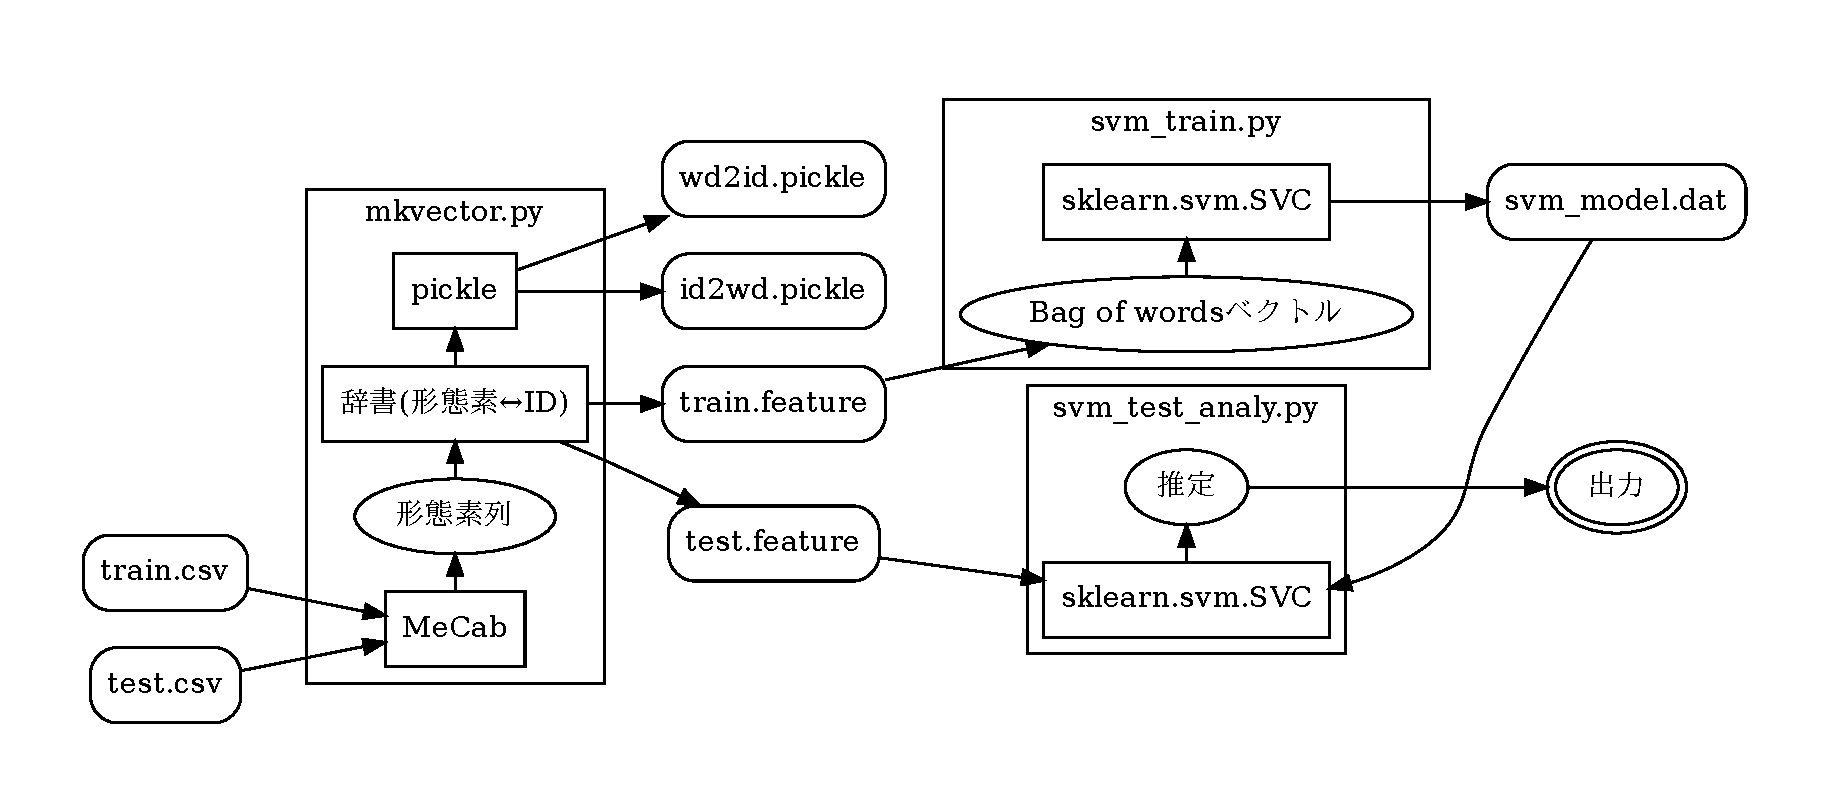
\includegraphics[width=16cm]{process.pdf}
  \caption{判別器の構成} \label{fig:process}
\end{figure}

判別器の構成は図\ref{fig:process}に示す通りである.

\verb|mkvector.py| では,1列目に正解ラベルが,2列目に文が書かれたCSVファイルを入力し,
MeCabによって形態素に分け,各形態素にIDを割り振った辞書を作る.
この辞書に形態素列を再び通し,
文を,ID$i$の形態素が現れるかどうかを第$i$成分としたBag-of-wordsベクトルとして,
疎ベクトルの形式で正解ラベルとともに \verb|.feature| ファイルに出力する.

\verb|svm_train.py| では,
\verb|train.feature| に出力された学習データのBag-of-wordsベクトルを
NumPyのベクトルに変換し,ラベルとともにscikit-learnのSVMに与えて学習する.
学習したモデルをpickleを用いて \verb|svm_model.dat| にdumpする.

\verb|svm_test_analy.py| では,\verb|svm_model.dat| をロードし,
\verb|test.feature| に出力されたテストデータのBag-of-wordsベクトルを
NumPyのベクトルに変換し,SVMで推定する.
推定結果とacculacyを出力する.

\section{出力}

出力結果の抜粋を以下に示す.

\begin{Verbatim}
num_axis= 3010
shape (175, 3010)
correct, estimated
0        0       a,婆さんはどこからとり出したか、眼をつぶった妙子の顔の先へ、一挺のナイフを突きつけました。
1        1       e,私は仕方がないので母親に貰ったお小遣いをふんぱつして、人力車に乗りました。
2        2       m,小川君は好奇心が起って溜まらなくなった。
******* (中略) *******
2        2       m,翌朝深淵の家へは医者が来たり、警部や巡査が来たりして、非常に雑※(「二点しんにょう+鰥
のつくり」、第4水準2-89-93)した。
1        1       e,数年以前から、いつもあんな苦し相な顔をして居ります。
0        0       a,五
0        1       a,そうしてこれが出来なければ、勿論二度とお父さんの所へも、帰れなくなるのに違いありません。
acccuracy= 0.903
\end{Verbatim}

学習データに3009種類の形態素が含まれたことから,
それ以外の形態素を未知のものとして1つの次元で表現し,
特徴ベクトルは3010次元のベクトルとなっている.

テストデータは175個の3010次元ベクトルが集まった行列としてSVMに入力され,
その推定結果が2列目に,正解ラベルが1列目に出力されている.
推定の結果,acculacyは0.903であった.

\end{document}
